\documentclass{beamer}
\usepackage{amsmath,amssymb,amsthm,array}
\usepackage{bm}
\usepackage{xltxtra}
\usepackage{multirow}
\usepackage{multicol}
\usepackage{algorithm}
\usepackage{algorithmic}
\usetheme{CambridgeUS}
\usecolortheme{beaver}
\usefonttheme{serif}
\setmainfont[Mapping=TeX-text]{GFS Neohellenic}
\setbeamertemplate{navigation symbols}{}
\title{A voting system case study:Pret-A-Voter}
\author{Panagiotis Grontas}
\date{26/06/2013}
\defbeamertemplate*{footline}{shadow theme}
{%
  \leavevmode%
  \hbox{\begin{beamercolorbox}[wd=.5\paperwidth,ht=2.5ex,dp=1.125ex,leftskip=.3cm plus1fil,rightskip=.3cm]{author in head/foot}%
    \usebeamerfont{author in head/foot}\insertframenumber\,/\,\inserttotalframenumber\hfill\insertshortauthor (\insertshortinstitute)
  \end{beamercolorbox}%
  \begin{beamercolorbox}[wd=.5\paperwidth,ht=2.5ex,dp=1.125ex,leftskip=.3cm,rightskip=.3cm plus1fil]{title in head/foot}%
    \usebeamerfont{title in head/foot}\insertshorttitle%
  \end{beamercolorbox}}%
  \vskip0pt%
}
\institute{$\mu\Pi\lambda\forall$  - CoReLab Crypto Group}


\setlength{\columnseprule}{0.4pt}
\begin{document}

\begin{frame}
\titlepage
\end{frame}

\section*{Elections With Receipts}

\begin{frame}[allowframebreaks]{Verifiable Elections With Receipts}

\begin{block}{Cryptographic Voting Receipts}
\begin{itemize}
\item Assure Voters that their vote is counted
\item While maintaining ballot secrecy and avoiding coercion 
\end{itemize}
\end{block}

\begin{block}{Advantages}
\begin{itemize}
\item Mathematically ensure election integrity
\item Allow software independence \cite{rivest2008notion}
\begin{itemize} 
\item Avoid trust on proprietary hardware
\item Detect errors early (at the polling station)
\item Rerun the elections without software
\end{itemize}
\end{itemize}
\end{block}

\begin{block}{Software independence}
A voting system is software independent if an undetected change or error in its software cannot cause an undetectable change or error in the election outcome. 
\end{block}
How: 
\begin{itemize}
\item Paper trail
\item Cryptography
\end{itemize}

\end{frame}

\begin{frame}{Voting with receipts}
\begin{itemize}
\item Input choices on the touch screen of the voting machine
\item Printer prints the receipt
\item Voter checks the printout
\item Accept or Change Vote
\item Mechanism for ballot secrecy
\item Receipt
\item Mechanism for receipt secrecy
\item Anonymization
\item Tallying
\item Verification: Web Bulletin Board to enter receipt SN and verify that it is included in the tally
\end{itemize}
\end{frame}

\begin{frame}{Visual Cryptography }
\begin{itemize}
\item Encrypt written material in a \textbf{perfectly secure} way
\item Decryption is done by human visual system
\item Ciphertext and secret key are two pages of papers
\item Ciphertext can be transmitted by fax or published
\item Secret key is printed on transparent paper
\item Each one on its own is indistinguishable from random noise
\item When placed on top of each other we have decryption
\item A visual one time pad
\begin{itemize}
\item Each page of cipher text is decrypted by its own transparency
\end{itemize}
\item Can be extended to $k \text{ of } n$ threshold secret sharing scheme \cite{naor1995visual}
\end{itemize}
\end{frame}

\begin{frame}{Receipts with Visual Cryptography - \cite{chaum2004secret}}
\begin{itemize}
\item Receipts consist of two layers laminated together
\item The printer prints the selection of the voter but does not conclude the job
\item Voter selects to keep top or bottom layer and then the printing concludes
\item Machine keeps the same layer in digital form
\item Neither layer is readable on its own, but both encode the vote
\item The other layer is destroyed by the voting personnel and the voting booth (securely?)
\end{itemize}
\end{frame}

\begin{frame}[allowframebreaks]{Encoding the vote with visual cryptography}
\begin{center}
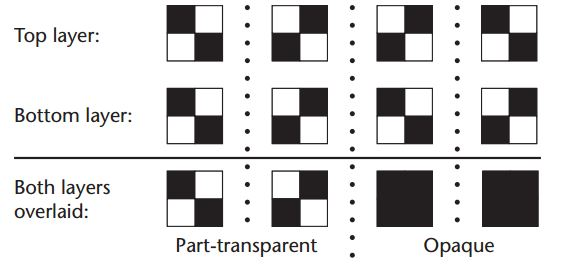
\includegraphics[scale=0.5]{visual}
\end{center}
\begin{center}
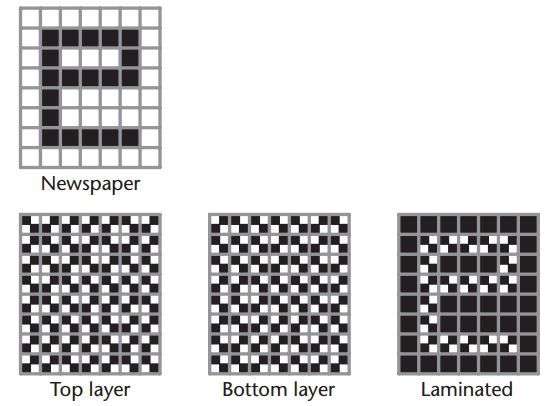
\includegraphics[scale=0.5]{visual1}
\end{center}
\end{frame}

\section*{PretAVoter with RSA}

\begin{frame}{PretAVoter - Introduction}
\begin{itemize}
\item End To End Verifiable Voting System
\item A design of ballots for electronic voting
\item Creator: Peter Ryan (University of Luxemburg) (2004)
\item Based on a previous cryptographic scheme by Chaum (2004)
\item Influenced a subsequent cryptographic scheme by Chaum 
\item First implementation by University of Surrey (2007)
\item Still in active development
\end{itemize}
\end{frame}

\begin{frame}{PretAVoter - Characteristics}
\begin{itemize}
\item Integrity
\item Voter Privacy
\item Receipt Freeness
\item Voter Verifiability
\item Voter Friendly
\item Modular: Can implement many cryptographic voting protocols (encryption, zero knowledge etc.)
\item Versatile: Can be used with many social choice functions
\item Requires supervised voting infrastructure
\end{itemize}
\end{frame}

\begin{frame}{Assumptions}
\begin{itemize}
\item Voter registration and authentication is outside the scope of the system
\item The ballot forms are properly managed (remain confidential, cannot be forged) between their creation and used
\item Voting occurs in a voting booth with the traditional privacy characteristics
\item There exists a tamper - free public bulletin board that can be used for verification 
\end{itemize}
\end{frame}

\begin{frame}[allowframebreaks]{The PretAVoter Ballot}
\begin{block}{Main idea}
The vote is recorded on a different frame of reference for each ballot.\\
As a result the system \textbf{encrypts the ballot not the vote}
\end{block}

 
\begin{itemize}
\item The ballot consists of two columns: one for the candidate list and one for the voter selection.
\item The candidate list is random for each ballot
\item The voter marks or ranks the candidates on his/her ballot
\item The candidate list \textbf{must} be disposed
\item The actual vote is the mark or rank that is recorded on the vote column
\item No encryption is needed, since the vote is useless without the candidate list
\item The vote column is used as a receipt for voter verifiability
\item Since the vote order is different, a source of voter bias is removed but compliance might be affected
\end{itemize}

\begin{center}
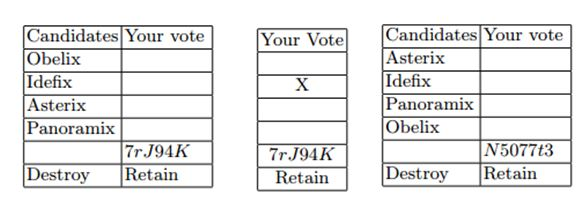
\includegraphics[scale=0.5]{ballot}
\end{center}

\begin{itemize}
\item There is a base ordering of a candidates
\item The ordering on each ballot is a permutation of the base 
\item The difference (offset) is encrypted and printed on each ballot
\item The encrypted value is called onion, referring to the processing of the ballot in the first version of the systems
\item The voting equipment records the index/ranking and transmits it along with the encrypted onion
\item Only the voter knows the order of the candidates that he voted on
\item \textbf{Extra bonus:} side channel attacks are side stepped
\begin{itemize}
\item No encryption takes place at the booth (the onion is created in advance)
\item The vote without the candidates is useless
\end{itemize}
\end{itemize}
\end{frame}

\begin{frame}[allowframebreaks]{Vote Processing}

\begin{enumerate}
\item Mixing
\item Decrypting
\item Tallying
\end{enumerate}

\begin{center}
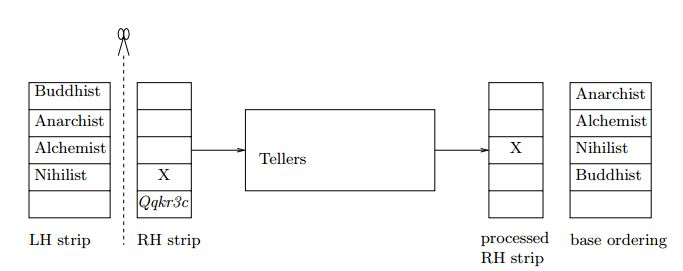
\includegraphics[scale=0.5]{voteprocessing}
\end{center}

\end{frame}

\begin{frame}[allowframebreaks]{Decryption Mixnet}

\begin{itemize}
\item $n$ voters
\item $m$ candidates
\item Each mix server performs 2 mixes

\begin{itemize}
\item $k$ mix servers 
\item $2k$ key pairs
\end{itemize}

\item Ballot generation - Layered Generation

\begin{itemize}
\item $2k$ random values $\{g_{i,j}\}_{0,0}^{n-1,2k-1}$ - germs - for each voter
\item the germs will be used for
\begin{itemize}
\item \textbf{randomised encryption}
\item Onion for ballot $i$: $D_{i,2k} = Enc(g_{i,2k-1},Enc(\cdots Enc(g_{i1},Enc(g_{i0},D_{i0})), \cdots))$ where $D_{i0}$ random value for initialisation
\end{itemize}
\begin{itemize}
\item \textbf{offset calculation}
\item $\theta_i = \sum_{j=0}^{2k-1} d_j \quad mod \quad m$ where $d_j=hash(g_{ij})$
\end{itemize}
\end{itemize}

\item Vote $i$ is a pair $(r_{i},D_{i,2k})$ where $r_i$ is the index of the marked candidate

\item Mix server operation
\begin{itemize}
\item Input $L_{2j}=\{r_i,D_{i,2j}\}_{i=0,j=k-1}^{n-1,0}$
\item Decrypt the onion with the private key $(g_ij,D_{ij})$
\item Apply the hash to the germ value of the onion $d_{ij}=hash(g_{ij})$
\item Calculate new shift  $r_{ij} = r_{i,j-1}-d_{ij}$
\item Sort the list by the value of the onions
\item Audit with RPC
\begin{center}
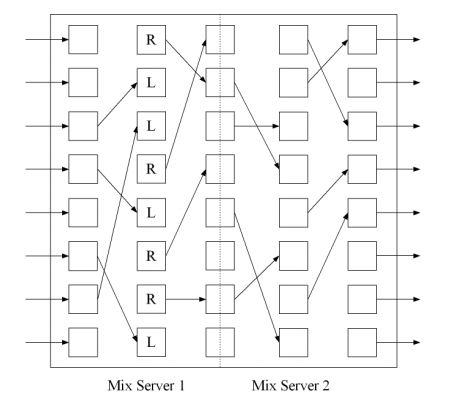
\includegraphics[scale=0.5]{auditrpc}
\end{center}
\end{itemize}

\end{itemize}

\end{frame}

\begin{frame}{Threats}
\begin{itemize}
\item Confidentiality of ballots, before elections. There is a need to trust the authority and the intermediates
\item Chain Voting: Coercion by smuggling a ballot, pre-voting, and require a replacement ballot
\item Kleptographic Channels: Choose special values of cryptographic variables in order to leak information to a colluding party
\begin{itemize}
	\item Tagging attack in mixnets
\end{itemize}
\end{itemize}
\textbf{Common Theme:} Too much trust in a single authority \\
\textbf{Solution:} Distributed Generation of Ballots
\end{frame}

\section*{PretAVoter with ElGamal}

\begin{frame}[allowframebreaks]{Distributed Generation Of Ballots}

\begin{itemize}
\item The ballot forms will be generated by $l$ entities called \textit{clerks}
\item Each clerk contributes to the generation of a common encrypted seed
\item The candidate list is constructed from the seed
\item To reveal the seed values all clerks must be corrupted
\item Encryption using exponential ElGamal (also works for RSA)
\item Tellers conduct tallying using a reencryption mixnet
\end{itemize}

\begin{block}{Operation}
\begin{itemize}
\item Generate 2 encrypted \textit{'onions'}:

\item $onion_L$ 
\begin{itemize}
\item will create the random candidate list
\item will be read (decrypted) by the voting machine in order to display the candidates to the voter
\end{itemize}

\item $onion_R$ 
\begin{itemize}
\item will be used for voter verifiability
\item and reconstruction of the candidate list
\end{itemize}

\end{itemize}
\end{block}

\begin{block}{Parameters}
\begin{itemize}
\item $p,q$ safe primes
\item $\alpha, \gamma$ generators of $\mathbb{Z}_q^*$
\item $\beta_T$ the public key of the tellers
\item $\beta_R$ the public key of the vote recording machines
\end{itemize}
\end{block}

\begin{block}{Clerk $C_0$}

\begin{itemize}
\item Generate a batch of initial seeds $s_i^0$ - one for each ballot
\item Create encryption with randomness $x_i^0,y_i^0$ for 
 
\item voting machine $E_{R}(\gamma^{ - s_i^0},x_i^0)=(\alpha^{x_i^0},\beta_R^{x_i^0} \cdot \gamma^{ - s_i^0})  $ 
\item teller $E_{T}(\gamma^{ - s_i^0},y_i^0)=(\alpha^{y_i^0},\beta_T^{y_i^0} \cdot \gamma^{ - s_i^0})$  
 
\end{itemize}
\end{block}

\begin{block}{Clerk $C_l$}
\begin{itemize}
\item Receive batch of onions from previous clerk
\item Generate fresh randomness 
\item Perform reencryption and shuffle
\end{itemize}
\end{block}

\begin{block}{Final onions}
\begin{itemize}
\item $onion_L=E_{R}(\gamma^{ - \sum_i s_i},\sum_i x_i)$
\item $onion_R=E_{T}(\gamma^{ - \sum_i s_i},\sum_i y_i)$ 
\end{itemize}
\end{block}
\begin{center}
\begin{center}
\emph{Correct operation $\Rightarrow$ the 'messages' match.}
\end{center}
\end{center}
\end{frame}

\begin{frame}[allowframebreaks]{Voting with distributed ballots}
\begin{itemize}
\item The onions are stored in encrypted form and are presented to the voter on the ballot form
\begin{center}
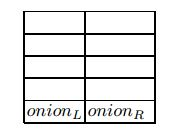
\includegraphics[scale=0.3]{distCandList.jpg}
\end{center}
\item Device reads and decrypts the left hand onion $s$ is revealed
\item The candidate permutation is reconstructed as a function of $s$
\item The device should not see the right onion
\end{itemize}
\begin{block}{Voting}
\begin{itemize}
\item The voter now faces a classical ballot
\item Marks candidate index
\item Embed selected candidate index into seed by reencryption
$vote=E_{T}(\gamma^{r - \sum_i s_i},\sum_i y_i)$
\item Mixing proceed as usual
\item Decryption: plaintexts are of the form $\gamma^{r - \sum_i s_i}$
\item Solve discrete logarithm
\item Select seeds so that the exponent is not too large and the search space is bounded
\item \textbf{Solution}: Use Paillier Cryptosystem
\end{itemize}
\end{block}
\end{frame}
 
\section*{STV Voting with PretAVoter}

\begin{frame}[allowframebreaks]{Overview of STV Voting}
\begin{block}{Objective:}
Reduce vote waste, for candidates that cannot win the election
\end{block}

\begin{itemize}
\item Each voter gets a single vote, but 'this vote' can be used by many candidates
\item When a candidate is eliminated, 'his' votes are transferred
\item Each voter ranks candidates
\item Ranking selects the candidates to receive the votes in case favourites are eliminated
\item \textbf{Tallying}
\begin{itemize}
\item Partition ballots according to the first choice of the voter
\item The candidate with the fewest votes is eliminated
\item His votes are transferred according to the second choices
\item Repeat until there is only one candidate
\end{itemize}
\end{itemize}

\begin{block}{Remarks}
\begin{itemize}
\item \textbf{Quotas:} The number of votes that assure election
\item If a candidate has reached the quota, he cannot be eliminated
\item But the surplus of votes has to be transferred, as well
\item The voter should not provide a complete ranking of the candidates.
\item A ballot with all the candidates eliminated is discarded
\end{itemize}
\end{block}

\begin{block}{Useful Characteristics}
\begin{itemize}
\item \textbf{Unused Preferences:} Some of the preferences might not be used, since the winner might get declared earlier.
\item \textbf{Transfer history} is irrelevant. We are not interested for the previous candidates since they are eliminated
\item \textbf{Lazy evaluation} can be applied. We can work on the candidates one by one.
\end{itemize}
\end{block}

\begin{block}{Difficulties}
\begin{itemize}
\item \textbf{The italian attack} Many preferences introduct a covert channel, as lower ranked preferences can be used to identify the voter
\end{itemize}
\end{block}

\end{frame}

\begin{frame}[allowframebreaks]{Incorporating STV into PretAVoter \cite{heather2007implementing}}
\begin{block}{Attempt 1}
\begin{itemize}
\item Encode a partial ranking in the vote
\item Keep the cyclic shift
\item But this might leak too much information because it preserves the relations found in the canonical ordering
\item An example:
\begin{center}
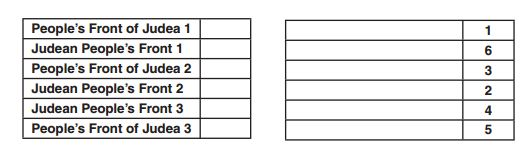
\includegraphics[scale=0.5]{stv.jpg}
\end{center}
\item We must embed a complete permutation
\end{itemize}
\end{block}

\begin{block}{Attempt 2 - ElGamal}
\begin{itemize}
\item Encode a permutation in the ElGamal exponent in a way that addition/multiplication yields permutation composition
\item Cannot be done
\end{itemize}
\end{block}

\begin{block}{Attempt 3 - RSA onions}
\begin{itemize}
\item Each layer encodes a permutation that can be recovered and applied
\item \textbf{Problems}
\begin{itemize}
\item It is evident how many choices were made
\item This can be used to partition ballots and leak information
\item No random padding can be added, since it will affect the election results
\item The candidates that were not ranked can be used as a covert channel (Italian attack)
\end{itemize}
\end{itemize}
\end{block}


\begin{block}{Solution:Multi valued reencryption mixes}
\begin{itemize}
\item Encode the vote as a sequence of cryptograms $\{ c_1, \cdots, c_k \} $ that decrypts to a candidate index
\item The order of the cryptograms reflects the ranking of the candidates by the voter, ie $c_1$ is the encryption of the index of the favourite candidate
\item A dummy candidate 'STOP' id included that marks the end of the user ranking
\item A complete ranking is given by using a random permutation of the remaining candidates
\item \textbf{Lazy Tallying:} First decrypt the heads
\item First preferences are counted
\item If a candidate is eliminated then the head is appended at the end, an anonymising mixnet is run and the heads are again decrypted
\item Stop when a winner (a candidate with more than half the votes) is found
\end{itemize}
\end{block}

\end{frame}

\begin{frame}[allowframebreaks]{STV with PretAVoter:An example}

\begin{block}{Ballot Form}
\begin{itemize}
\item Each ballot form contains a signed hash
\item Hash serves as a key to lookup $k+1$ onions
\begin{itemize}
\item The first $k$ correspond to the candidates $\{ i, z \}_{PK_{T}}, i=1 \cdots k$ and are presented in random order
\item The last is the encryption of the stop candidate  $\{ 0, z \}_{PK_{T}}$
\end{itemize}
\end{itemize}
\end{block}
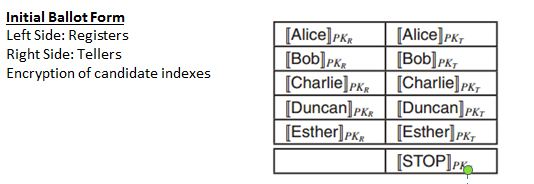
\includegraphics[scale=0.5]{stv1.jpg}


\begin{itemize}
\item Distributed Ballot Generation
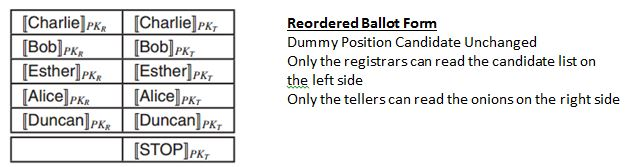
\includegraphics[scale=0.5]{stv2.jpg}
\item Each ballot can be printed by a subset of registrars after being retrieved from a bulletin' board
\end{itemize}

\begin{block}{Voting}
Voter sees the decrypted ballot form, without the 'STOP' candidate and ranks the candidates (partially)
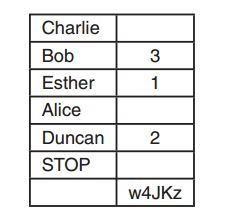
\includegraphics[scale=0.5]{stv3.jpg}
Booth sends the ranking and the hash to the bulletin board
\end{block}

\begin{block}{PostVoting Bulletin Board Actions}
\begin{itemize}
\item First Available ranking is assigned to 'STOP' candidate
\item Rest of empty voters are filled from top to bottom
\item Use the hash to retrieve candidate list
\item Sort Based on ranking
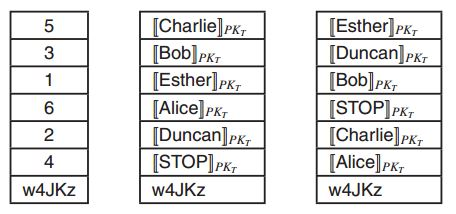
\includegraphics[scale=0.5]{stv4.jpg}
\end{itemize}
\end{block}

\begin{block}{Anonymising and tallying}
\begin{itemize}
\item Apply STV
\item Decrypt candidates one at a time, until stop is reached
\item After each decryption, another round of anonymisation occurs
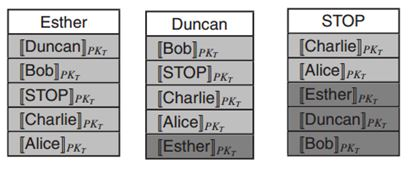
\includegraphics[scale=0.5]{stv5.jpg}
\end{itemize}
\end{block}

\end{frame}

\section*{Condorcet Voting with PretAVoter}

\begin{frame}{Condorcet Voting}
\begin{itemize}
\item The voter provides a full ranking of the candidates
\item All candidates engage in pairwise comparisons (duels)
\item The winner of each dual is the candidate that is preferred by the majority of the voters 
\begin{block}{An example - duel between the candidates $c_A$ and $c_B$}
For each ballot $b$ do \\
\hspace{10mm}	 if $c_A$ is ranked higher than $c_B$ in $b$ then \\
\hspace{20mm}		 	$w_A \leftarrow w_A + 1$ \\
\hspace{10mm} 	 else \\
\hspace{20mm}    $w_B \leftarrow w_B + 1$ \\
$duel-winner \leftarrow$ candidate with $w=max(w_A,w_B)$
\end{block}
\item The winner of the election is the one that wins \textbf{all} the duels
\item There might not be a winner, so a completion method is used (but this is a backend issue)
\end{itemize}
\end{frame} 

\begin{frame}{Ballots for Condorcet Voting \cite{Clarkson05}}
\begin{itemize}
\item For $c$ candidates we have $\frac{c (c-1)}{2} \dashrightarrow O(c^2)$ ballots
\item Each ballot is a $yes/no$ choice for candidates $i,j$
\item A yes choice indicates preference for candidate $i$ over candidate $j$
\item Each yes/no ballot has its own onion $<i,j>$
\item Layered construction of onions for use in decryption mixnet
\item Each voter submit   $c \times c$ votes with the preferences and the onions
\item The vote is run through a decryption mixnet for anonymisation
\item \textbf{Remark}: There can be no correlation that all $c^2$ votes belong to the same voter
\item A summation matrix is used to declare the winner 
\end{itemize}
\end{frame}

\begin{frame}[allowframebreaks]{References}
\begin{tiny}
\nocite{*}
\bibliographystyle{alpha}
\bibliography{pretAVoter}
\end{tiny}
\end{frame}

 
\end{document}
